\documentclass[UTF8,zihao=-4,fontset=windows]{ctexart}
\usepackage[a4paper,margin=22mm]{geometry}
\usepackage{booktabs,tabularx,array,graphicx,amsmath,xcolor,float,tikz,pgfplots}
\pgfplotsset{compat=1.18}\usepackage[hidelinks]{hyperref}
\setlength{\parskip}{.45em}\setlength{\parindent}{0pt}\emergencystretch=3em
\def\fitlabel{拟合集总体召回}\def\controlname{同轮对照}\def\treatmentname{实验方案}
\def\objectlabel{内部 Dead 对象数}\def\retained{保留}\def\gained{新增}\def\lost{丢失}\def\missed{共同漏检}\def\seedname{种子}
\def\roundxlabel{Dead命中变化：处理组减同轮对照}\def\seedlabel{种子}
\def\fractionlabel{比例}\def\deadlabel{Dead召回}\def\overalllabel{总体召回}\def\precisionlabel{精度}
\def\fitdead{拟合Dead召回}\def\auditdead{审计Dead召回}
\title{\bfseries 核中心定位：从逐轮实验到逐对象诊断\\\large 阶段报告7}\author{bdd26 research}\date{10 November 2026}\begin{document}\maketitle\tableofcontents\newpage
\section{研究问题与本阶段结论}
模型在每张病理图中为细胞核给出中心点。审计集有522张图、12,250个核，其中145个内部 Dead 核分布在11张图中；拟合集为2,134张图。预测点与标注中心按3像素半径一对一匹配。总体召回衡量找到的全部标注核比例；Dead召回聚焦标注为Dead的子集；精度衡量预测点中成功匹配的比例。

本阶段的关键线索来自多次方向不同的实验。P17显示从头训练模型连拟合图的覆盖也很低；P19显示固定轮数下加大有效批量减少优化更新并降低拟合覆盖；P20显示放大输入可以增加部分Dead命中，但训练成本约增至4.3倍；P21的语义辅助头改善拟合却降低审计总体覆盖。P22全层适配同时增加命中并减少额外点，收益最清楚；逐对象结果又展示了新增、丢失与共同漏检。P23的参数平均只带来少量变化；P24较高编码器学习率稳定提高精度，却在不同图和种子上产生不同的Dead变化；P25分层适配明显改善总体找点；P26参数锚定则使总体召回与精度下降。
\begin{figure}[H]\centering\begin{tikzpicture}
\begin{axis}[xbar, width=.9\linewidth,height=9cm, xmin=-40,xmax=25,
 xlabel={\roundxlabel}, symbolic y coords={P25,P24,P23,P22,P21,P20,P19,P18,P17},
 ytick=data, legend style={at={(.5,1.1)},anchor=north,legend columns=2},
 grid=major,bar width=5pt]
\addplot coordinates { (7,P25) (11,P24) (1,P23) (18,P22) (1,P21) (13,P20) (-9,P19) (-1,P18) (-30,P17) };
\addplot coordinates { (10,P25) (-2,P24) (3,P23) (20,P22) (-5,P21) (6,P20) (0,P19) (3,P18) (-36,P17) };
\legend{\seedlabel\ 19,\seedlabel\ 1}
\end{axis}\end{tikzpicture}
\caption{每轮处理组相对同轮对照的Dead命中净变化，分母145；P22在两个种子均显示最大的增量。}\end{figure}
\section{P17--P21：从拟合能力到图像尺度}
\subsection{P17：高精度背后的覆盖收缩}
从头训练的卷积模型K在种子19只提出1,795个点，其中1,709个匹配，精度95.21\%；同轮UNI对照提出10,644个点、匹配7,285个，精度68.44\%。K有198/522张图完全没有预测，对照为22张。K的拟合总体召回仅14.41\%和11.92\%，审计总体召回13.95\%和11.89\%。Dead命中为30/31，对照为60/67。这里最直接的问题是大量区域缺少候选点；精度高来自仅保留少量较容易的预测。

\subsection{P18：增加RGB通路改善拟合，组织收益互相抵消}
RGB残差H保留UNI编码器。种子19的拟合总体召回由97.43\%升至98.52\%，审计匹配数从7,172增至7,361；种子1增加37个审计匹配。Dead却分别从71变70、64变67。种子19的肺图净增4个Dead，结肠图净减5个；种子1肺和结肠各净增2个，宫颈净减2个。附加原图通路扩大了总体覆盖，组织间的增减决定了稀有目标的最终净变化。

\subsection{P19：更大的有效批量改变优化步数}
有效批量由16增至32，每轮AdamW更新从134次降到67次。130轮后，种子19拟合总体召回从97.37\%降至94.74\%，种子1从97.91\%降至94.10\%；对应Dead从66变57、63保持63。种子1结肠净增5个，食管净减4个、肺净减2个。拟合覆盖下降与更新次数减半共同出现，说明固定轮数下的优化进度值得关注。物理批量相同，纯训练时间仅缩短约1.5--1.9\%。

\subsection{P20：放大输入让一部分目标更容易检出}
将256图插值到512后编码，种子19 Dead由66升至79，种子1由69升至75。种子19肺部增加10、结肠增加5，宫颈减少2；种子1肺部增加4、宫颈增加5，食管减少3。较小Dead的命中分别为7到9和8到7。拟合Dead从629/627升至653/655，而审计总体匹配分别仅增加3个和减少244个。U臂纯训练约17.1--17.3小时，同轮对照约4小时。尺度改变了局部编码与候选分布，收益和成本需要一起考量。

\subsection{P21：训练期五类中心辅助头}
辅助头A使种子19审计匹配数从7,300降至7,132，种子1从7,389降至7,241；Dead分别为64到65、70到65。种子1食管图从7/8降到2/8，肺的一张图由11降到7；小Dead从10/32降到5/32。两种子拟合匹配都增加，审计匹配却减少，表明辅助监督改变了共享特征上的取舍。

图中的肺图1025包含38个标注核、25个内部Dead。种子19对照预测38点、匹配29个；A预测39点、匹配27个。绿色位置在两图中可直接比较；新增的红圈显示原来找到的部分核变成漏检，橙圈显示额外预测。该图把总体变化落实到具体空间位置。
\begin{figure}[H]\centering\begin{tikzpicture}
\begin{axis}[ybar,bar width=12pt,width=.9\linewidth,height=6cm,ymin=0,ymax=1.08,
 ylabel={\fitlabel},symbolic x coords={P17,P19,P20,P22},xtick=data,grid=major,
 legend style={at={(.5,1.14)},anchor=north,legend columns=2},point meta=explicit symbolic]
\addplot coordinates {(P17,.9789) [0.979] (P19,.9737) [0.974] (P20,.9785) [0.979] (P22,.9777) [0.978]};
\addplot coordinates {(P17,.1441) [0.144] (P19,.9474) [0.947] (P20,.9976) [0.998] (P22,.9882) [0.988]};
\legend{\controlname,\treatmentname}\end{axis}\end{tikzpicture}\caption{种子19拟合总体召回：P17、P19、P20和P22各自的对照与处理。}\end{figure}
\begin{figure}[H]\centering\begin{tikzpicture}
\begin{axis}[ybar,bar width=16pt,width=.9\linewidth,height=6cm,ymin=0,ymax=1.1,
 ylabel={\fractionlabel},symbolic x coords={C19,U19,C1,U1},xtick=data,grid=major,
 legend style={at={(.5,1.14)},anchor=north,legend columns=2}]
\addplot coordinates {(C19,.95884) (U19,.99543) (C1,.95579) (U1,.99848)};
\addplot coordinates {(C19,.45517) (U19,.54483) (C1,.47586) (U1,.51724)};
\legend{\fitdead,\auditdead}\end{axis}\end{tikzpicture}\caption{P20 拟合与审计Dead召回；C为256输入，U为插值到512后编码。}\end{figure}
\begin{figure}[H]\centering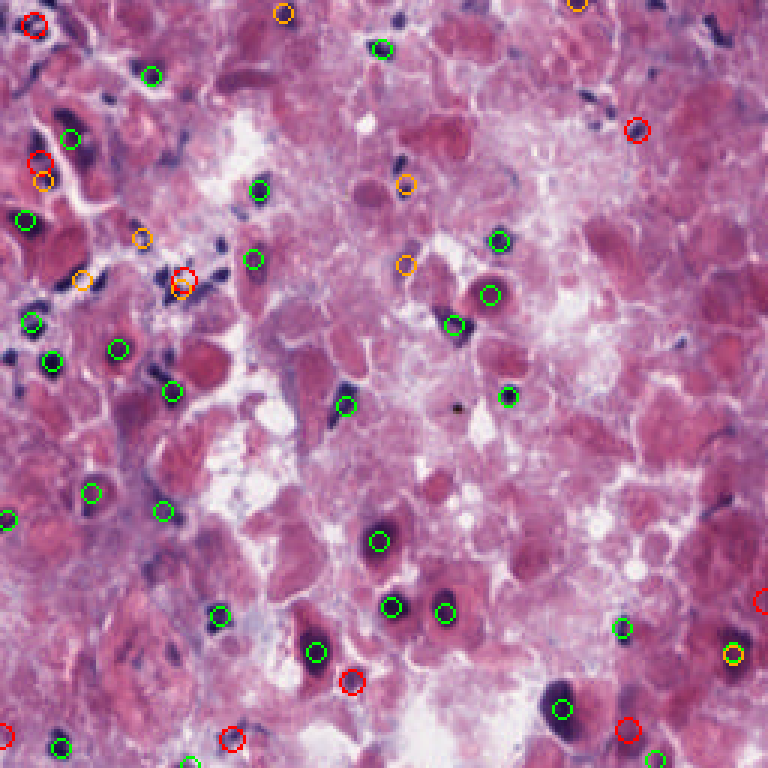
\includegraphics[width=.47\linewidth]{assets/casebook/p21_c_1025.png}\hfill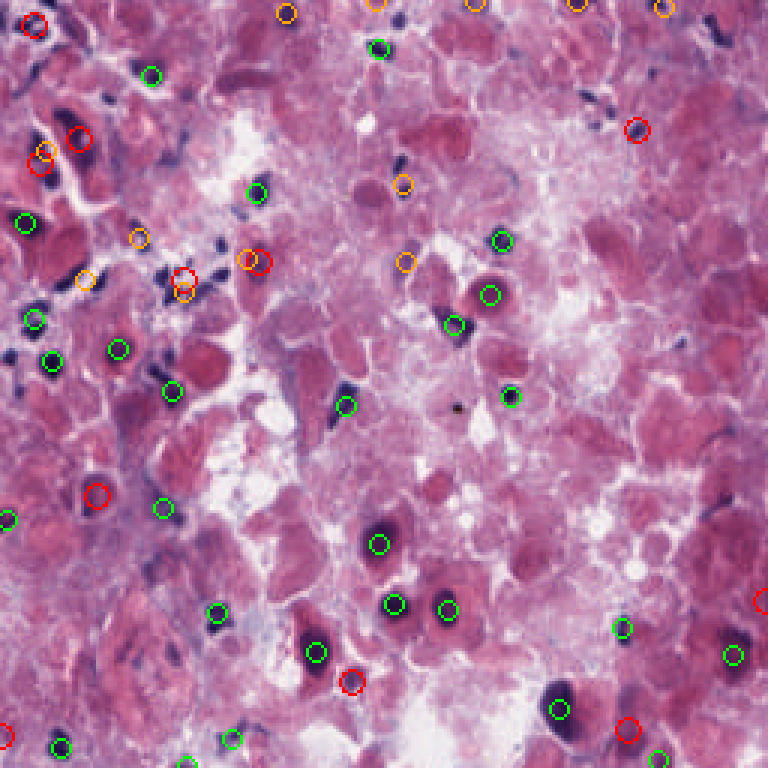
\includegraphics[width=.47\linewidth]{assets/casebook/p21_a_1025.png}\caption{P21肺图1025，左C、右A。绿：匹配；红：漏检；橙：额外点。}\end{figure}
\section{P22：全层适配找回了哪些核？}
对照C训练UNI最后12层，M训练24层。种子19 Dead由67升至85，种子1由62升至82；总体召回分别提高6.02和6.15个百分点，精度提高3.64和3.46个百分点。种子19多产生488个候选，同时多匹配738个核，额外点减少250个；种子1分别为候选增加542、匹配增加753、额外点减少211。全层适配同时增加覆盖和改善候选质量。纯训练时间约增加42--43\%，峰值显存由4.05增至6.75 GiB。

145个Dead的逐对象对照给出更细的结果：种子19保留55个原有命中、新找到30个、丢失12个、两组均漏48个；种子1依次为56、26、6、57。种子19的肺图净增12个、宫颈净增7个；结肠新增5个又丢失5个，净变化为0。小Dead两种子均从7/32增至11/32。下面三张局部图把这些变化对应到具体核。

每张局部图左、中、右依次为原图、C匹配图、M匹配图；白黑双环标出同一GT核，绿圈为匹配、红圈为漏检、橙圈为额外点。原图为80×80像素局部并作最近邻放大。模型响应取标注中心3像素范围内最大值，固定阈值为0.5。
\begin{figure}[H]\centering\begin{tikzpicture}
\begin{axis}[ybar,bar width=14pt,width=.9\linewidth,height=6cm,ymin=0,ymax=65,
 ylabel={\objectlabel},symbolic x coords={Retained,Gained,Lost,Missed},xtick=data,
 xticklabels={\retained,\gained,\lost,\missed},grid=major,nodes near coords,
 legend style={at={(.5,1.14)},anchor=north,legend columns=2}]
\addplot coordinates {(Retained,55) (Gained,30) (Lost,12) (Missed,48)};
\addplot coordinates {(Retained,56) (Gained,26) (Lost,6) (Missed,57)};
\legend{\seedname\ 19,\seedname\ 1}\end{axis}\end{tikzpicture}\caption{P22逐GT对象的四种状态，两个种子各合计145个。}\end{figure}
\begin{figure}[H]\centering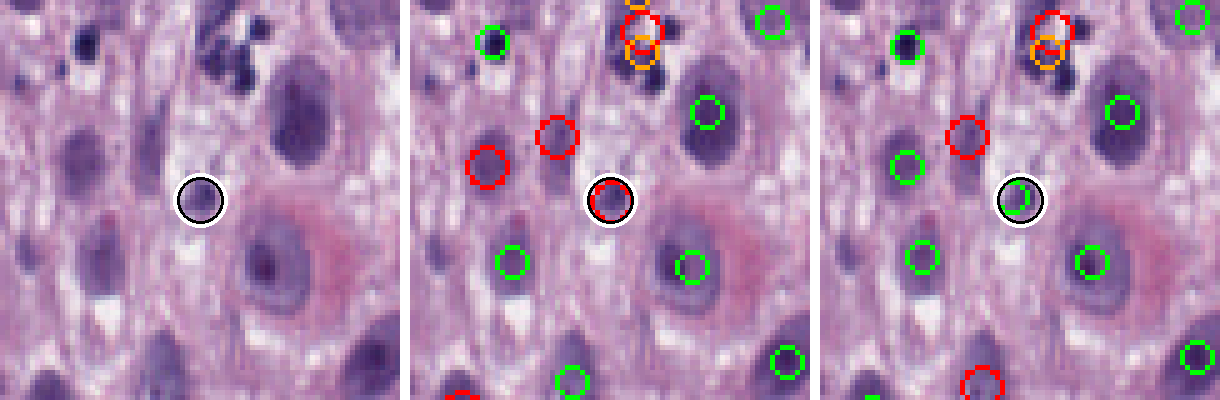
\includegraphics[width=.98\linewidth]{assets/casebook/recovered_1037.png}\caption{肺图1037、对象67（行98、列180，面积65像素）：C局部响应接近0，M升至0.792，状态由红色漏检变为绿色匹配。}\end{figure}
该核较小，邻近深染结构；放大后可看到C在该位置没有形成有效候选，M在相同位置产生匹配。
\begin{figure}[H]\centering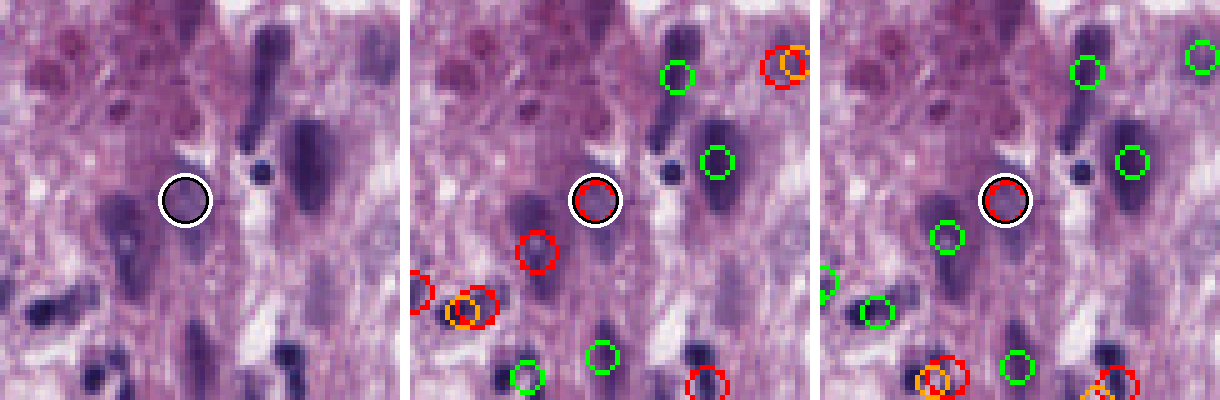
\includegraphics[width=.98\linewidth]{assets/casebook/missed_1037.png}\caption{肺图1037、对象57（行43、列37，面积214像素）：C响应接近0，M升至0.446，两个输出均显示红色漏检。}\end{figure}
该核周围有多个深染结构。M的局部响应上升，但仍低于0.5，因而该位置没有进入最终匹配。
\begin{figure}[H]\centering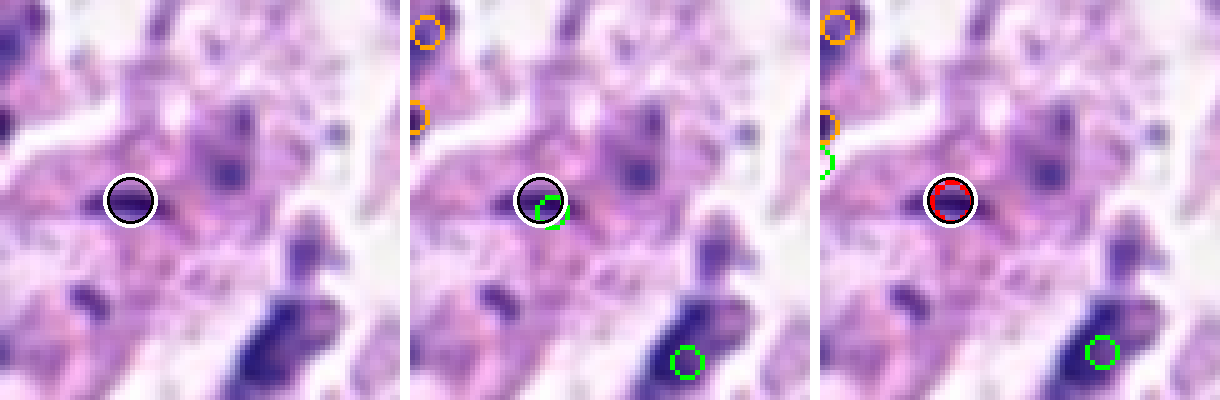
\includegraphics[width=.98\linewidth]{assets/casebook/lost_0776.png}\caption{结肠图776、对象7（行148、列26，面积137像素）：C响应0.835并匹配，M响应0.146并漏检。}\end{figure}
这枚核在C输出中有绿色匹配，M输出在同一标注处出现红圈。全层适配会改变已经找到的对象；逐对象得失揭示了净变化背后的交换。
\section{P23--P26：参数平均、学习率与参数锚定}
\subsection{P23：EMA主要保留已有结果}
每个种子的一条轨迹产生最终权重C和0.999指数平均权重E。Dead命中由69到70、60到63；小Dead在四个输出中均为6/32。种子19逐对象记录显示69个原命中全部保留，1个低响应对象变为匹配，72个仍为低响应。改善落在肺图1025的1个对象；种子1的增量分别落在结肠776、结肠1482和宫颈1756。平均参数主要平滑已有响应，最小目标的漏检格局保持明显。

\subsection{P24：较高学习率改善精度，局部收益各异}
最后12层学习率从 $10^{-5}$ 提至 $3\times10^{-5}$。两种子的精度分别由0.688升至0.732、0.694升至0.731；候选减少589/471个，同时全体匹配增加29/38个。Dead分别由67升至78、68降至66。小Dead均由7/32升至11/32；较大Dead的变化分别为净增7、净减6，因此种子1的小核收益被其他对象的减少抵消。

固定肺图1037中Dead命中在两种子分别增加5和3；同为肺图的1025却分别减少1和3。宫颈图1756两个种子的变化为+2和-4。下图展示种子19的1037：右侧L图中部分原红圈转为绿色，同时仍有红圈与橙圈；相邻核周围的响应变化各异。

\begin{figure}[H]\centering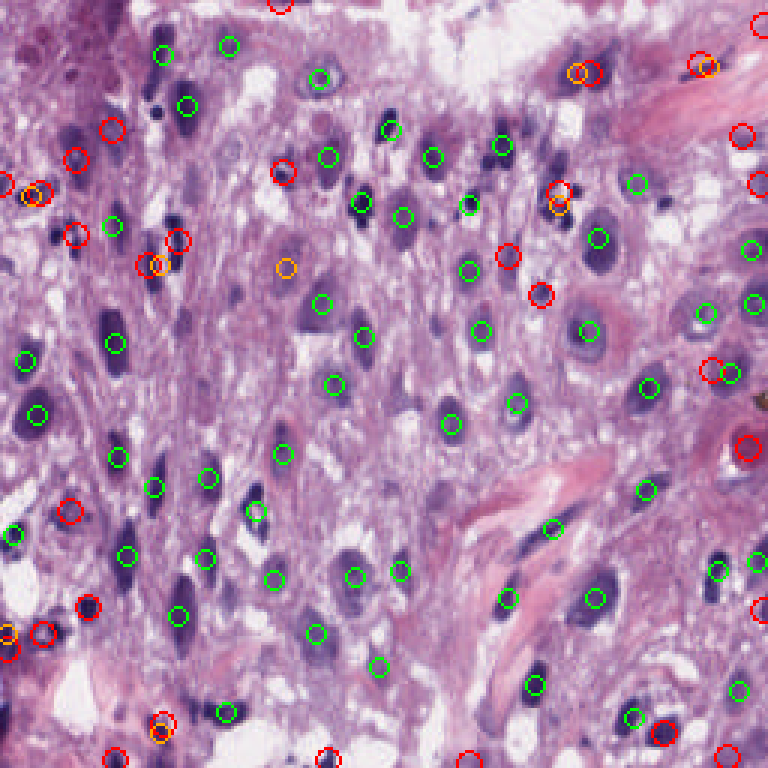
\includegraphics[width=.47\linewidth]{assets/casebook/p24_c_1037.png}\hfill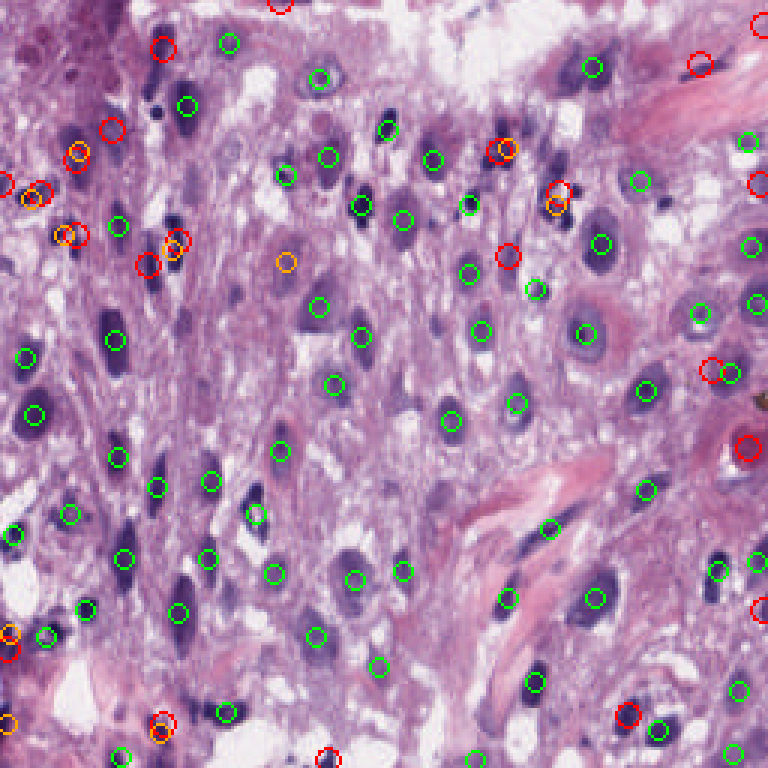
\includegraphics[width=.47\linewidth]{assets/casebook/p24_l_1037.png}\caption{P24肺图1037，左C、右L，种子19。绿为匹配、红为漏检、橙为额外点。}\end{figure}
\subsection{P25：全层分层速率改善全体找点}
24层采用由低到高的分层学习率。两种子的总体召回从0.590/0.598升至0.650/0.640，精度从0.690/0.692升至0.744/0.742；Dead命中从69到76、65到75。分别多匹配741和512个核，额外点减少510和544个。肺图1037由10到15、10到16，结肠图1482由15到9、14到10。组织之间的相反变化解释了总体Dead净增低于肺部单独增量。

\subsection{P26：约束编码器接近预训练参数}
四项均完成130轮。种子19的Dead从67到69，种子1从64到66；锚定组总体召回为0.571/0.569，对照为0.584/0.596；锚定组精度0.679/0.688，对照0.697/0.693。两个种子的配对Dead变化均为2/145，原始区间分别为 $[-0.006173,0.053793]$ 与 $[-0.071429,0.061224]$。锚定在本次设置下抑制了总体覆盖和精度，Dead变化很小。

\section{综合分析：漏检发生在什么环节}
P22四个模型的Dead漏检中，94.87\%--97.59\%属于局部低响应：GT中心3像素范围内最大值低于0.5。种子19 C/M的低响应分别为74/57，定位或NMS漏检为4/3。与局部图中的对象57相对应，模型先需要在目标位置形成足够强的中心响应；对象67展示响应增强后可以形成匹配，而结肠对象7展示另一处响应会同时减弱。这些对象提供了下一步诊断的具体位置：检查局部特征与训练图中相似形态的响应，并比较组织背景下的中心概率分布。

本报告的配对数字均以同轮、同种子对照计算；审计图及对象标注的身份和源文件见随附数值索引。\texttt{NUMBER\_SOURCES.md}给出数据路径、匹配定义和图像来源。
\begin{figure}[H]\centering\begin{tikzpicture}
\begin{axis}[ybar,bar width=9pt,width=.90\linewidth,height=7cm,ymin=0,ymax=.8,
 ylabel={\fractionlabel},symbolic x coords={C19,R19,C1,R1},xtick=data,grid=major,
 legend style={at={(.5,1.16)},anchor=north,legend columns=3}]
\addplot coordinates {(C19,.462069) (R19,.475862) (C1,.441379) (R1,.455172)};
\addplot coordinates {(C19,.583673) (R19,.570857) (C1,.596245) (R1,.569224)};
\addplot coordinates {(C19,.697221) (R19,.678537) (C1,.692519) (R1,.688080)};
\legend{\deadlabel,\overalllabel,\precisionlabel}
\end{axis}\end{tikzpicture}
\caption{P26四跑审计：各种子对应一组C与R。}\end{figure}
\end{document}
